\section{Evaluation}
\label{sec:eval}
We want to evaluate and compare our implementations of the three different parallel solvers in \gob. Before comparing their performance with respect to evaluation time, we investigate if the parallelization results in a loss of precision.
The source repository of \gob\ contains more than 1400 regression tests. These are small programs focussed on testing various edge cases of the different features of the analyzer. We observe that for less than 0.5\% of the regression tests the parallelized solvers from~\autoref{sec:method:td_parallel} were less precise than the single-threaded solver we introduced in~\autoref{sec:background:td}. This loss of precision was non-deterministic, i.e., in some runs there was no loss of precision observed. Furthermore, when analyzing real-world programs like we do in the following sections, no loss of precision was observed in the warnings \gob\ produced. These warnings include but are not limited to notifications about thread-(un)save memory locations and dead lines of code. Thus, we believe that the parallelized solvers can be considered as precise as the single-threaded solver we compared them against. We note here that \gob\ typically uses an improved version of the single-threaded \ac{td} from this report and thus is even more precise in 32 of the regression tests.

  \subsection{Analysis speed}
  \label{sec:eval:speed}
  To evaluate the speed of the different solvers, we analyze several programs and compare the time of the analysis. We use two groups of programs for this evaluation. The first are a selection of the GNU core utility programs (coreutils)~\cite{gnuCoreutils}. Before analysis, these programs were combined, i.e., a single source code file was produced, that contains the original program together with the dependencies of other included files. The exact code files used can be found in the \gob\ benchmark repository~\cite{goblintBench} that contains benchmark programs for the analyzed.
  The second group are programs from the pthread folder of the \gob\ benchmark repository. These are programs that use threads more extensively than the coreutil programs, i.e., they use threads slightly more often and the spawned threads perform much more work. We included these programs, since the shared memory \ac{td} and the disjunct \ac{td} depend on threads being spawned in the analyzed program to add tasks that are solved in parallel.\\
  For comparison, we analyze each program once with the single-threaded \ac{td} from~\autoref{sec:background:td} as a baseline and twice with each of the parallelized \acp{td} from~\autoref{sec:method:td_parallel}, where one run was done with only the main thread working and one run with two worker threads. We do this, so we can compare the analysis time between the single-threaded \ac{td} and a certain parallelized \ac{td} in more detail, e.g., attribute differences in analysis time to the inherently different algorithms of the solvers or to the parallelization. Since the programs are different in size and general analysis time, we mainly focus on the \textit{speedup} as a metric. We calculate the speedup of the parallelized solvers with the following formula:
  \begin{equation*}
    \text{speedup(parallel solver)} = \frac{\text{time(baseline solver)}}{\text{time(parallel solver)}}
  \end{equation*}
  With this we get a value larger than 1, if the parallelized solver is faster and a value smaller than 1 if it is slower. The raw timing values are listed in the appendix in~\autoref{fig:timing_all}.

  \begin{figure}
    %TODO: Adapt Colors. !!!WATCH CAPTION!!!
    \centering
    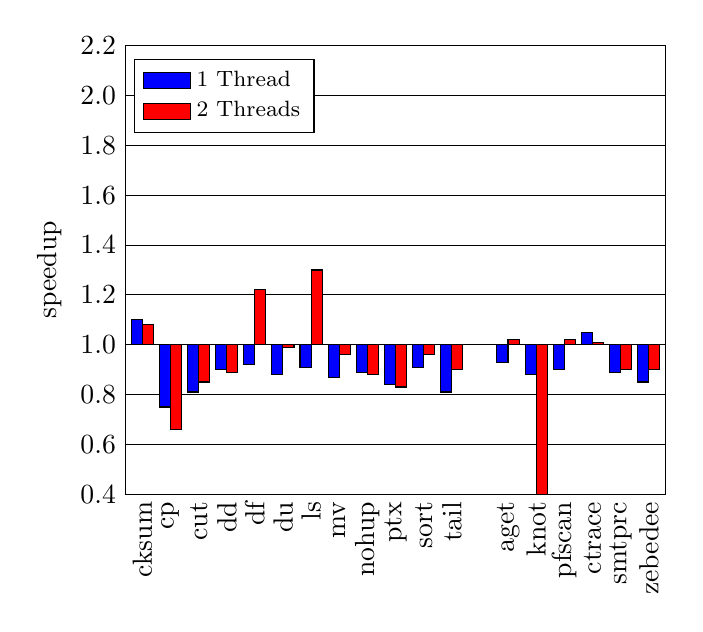
\begin{tikzpicture}
      \begin{axis}[ymin=-0.6, ymax=1.2, xmin=0, xmax=1, yticklabel=\empty, xticklabel=\empty, x tick style=transparent, y tick style=transparent]
          \draw (axis cs:0,-0.4) -- (axis cs:1,-0.4);
          \draw (axis cs:0,-0.2) -- (axis cs:1,-0.2);
          \draw (axis cs:0,0) -- (axis cs:1,0);
          \draw (axis cs:0,0.2) -- (axis cs:1,0.2);
          \draw (axis cs:0,0.4) -- (axis cs:1,0.4);
          \draw (axis cs:0,0.6) -- (axis cs:1,0.6);
          \draw (axis cs:0,0.8) -- (axis cs:1,0.8);
          \draw (axis cs:0,1) -- (axis cs:1,1);
      \end{axis}
      \begin{axis}[
          ybar=0pt,
          ymin=-0.6,ymax=1.2,
          ylabel = speedup,
          ytick pos = left,
          ytick distance = 0.2,
          ytick style = transparent,
          yticklabels={,0.4, 0.6, 0.8, 1.0, 1.2, 1.4, 1.6, 1.8, 2.0, 2.2},
          symbolic x coords={cksum, cp, cut, dd,df,du,ls,mv,nohup,ptx,sort,tail,,aget,knot,pfscan,ctrace,smtprc,zebedee},
          xtick=data,
          xtick style = transparent,
          x tick label style={rotate=90, xshift=5pt},
          enlarge x limits={abs=6pt},
          bar width = 4pt,
          legend style={at={(0.35,0.97)},anchor=north east, font=\footnotesize, legend cell align=left,},
          ]
          \addplot[ybar, fill=blue, area legend] coordinates {
            (cksum,0.1)
            (cp,-0.25)
            (cut,-0.19)
            (dd,-0.10)
            (df,-0.08)
            (du,-0.12)
            (ls,-0.09)
            (mv,-0.13)
            (nohup,-0.11)
            (ptx,-0.16)
            (sort,-0.09)
            (tail,-0.19)
            (aget,-0.07)
            (knot,-0.12)
            (pfscan,-0.10)
            (ctrace,0.05)
            (smtprc,-0.11)
            (zebedee,-0.15)
            }; 
          \addplot[ybar, fill=red, area legend] coordinates {
            (cksum,0.08)
            (cp,-0.34)
            (cut,-0.15)
            (dd,-0.11)
            (df,0.22)
            (du,-0.01)
            (ls,0.30)
            (mv,-0.04)
            (nohup,-0.12)
            (ptx,-0.17)
            (sort,-0.04)
            (tail,-0.10)
            (aget,0.02)
            (knot,-0.6)
            (pfscan,0.02)
            (ctrace,0.01)
            (smtprc,-0.10)
            (zebedee,-0.10)
            }; 
      \legend{1 Thread, 2 Threads}  
      \end{axis}
    \end{tikzpicture}
    \caption[Speedup of the stealing \ac{td}]{Speedup of the stealing \ac{td}. The runs with a single worker thread are shown in blue, while runs with two threads are represented by red bars. The twelve leftmost programs make up the coreutil group, while the six rightmost programs belong to the pthread group of programs. The run with two threads for the knot program resulted in a timeout of 900s}
    \label{fig:speedup_stealing}
  \end{figure}

  When investigating the results for the stealing \ac{td} from~\autoref{fig:speedup_stealing}, we notice, that in general this solver is slower or just as fast as the baseline. Furthermore, the difference between running this solver single threaded or with two worker threads is minimal. Interesting are the programs \texttt{df.c} and \texttt{ls.c} where the stealing \ac{td} achieved a speedup of 1.2 and 1.3 respectively. However, for the program \texttt{cp.c} it was significantly slower than the baseline. Unfortunately we are not able to explain the timeout for the \texttt{knot.c} program, as it terminated in a reasonable time when analyzed with a debugging configuration. We note here, that we only evaluate the stealing \ac{td} with the addition of revival, since the stealing \ac{td} is strictly faster with revival.

  \begin{figure}
    %TODO: Adapt Colors. !!!WATCH CAPTION!!!
    \centering
    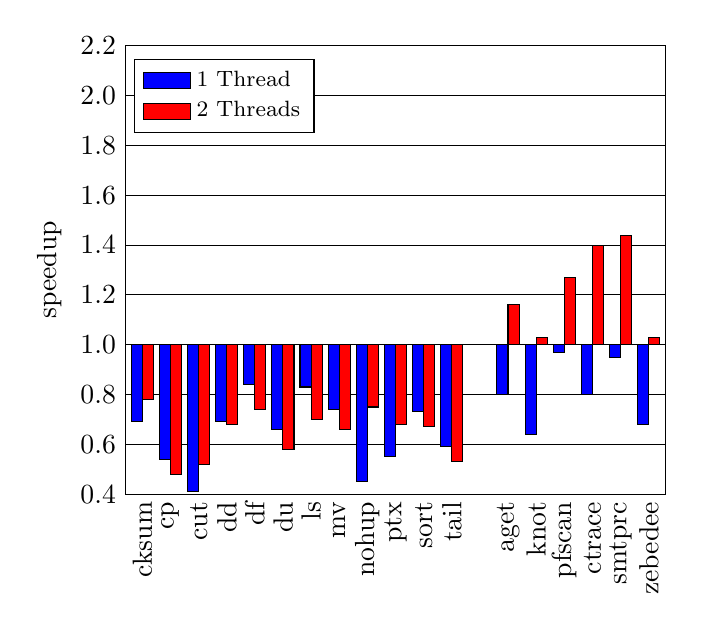
\begin{tikzpicture}
      \begin{axis}[ymin=-0.6, ymax=1.2, xmin=0, xmax=1, yticklabel=\empty, xticklabel=\empty, x tick style=transparent, y tick style=transparent]
          \draw (axis cs:0,-0.4) -- (axis cs:1,-0.4);
          \draw (axis cs:0,-0.2) -- (axis cs:1,-0.2);
          \draw (axis cs:0,0) -- (axis cs:1,0);
          \draw (axis cs:0,0.2) -- (axis cs:1,0.2);
          \draw (axis cs:0,0.4) -- (axis cs:1,0.4);
          \draw (axis cs:0,0.6) -- (axis cs:1,0.6);
          \draw (axis cs:0,0.8) -- (axis cs:1,0.8);
          \draw (axis cs:0,1) -- (axis cs:1,1);
      \end{axis}
      \begin{axis}[
          ybar=0pt,
          ymin=-0.6,ymax=1.2,
          ylabel = speedup,
          ytick pos = left,
          ytick distance = 0.2,
          ytick style = transparent,
          yticklabels={,0.4, 0.6, 0.8, 1.0, 1.2, 1.4, 1.6, 1.8, 2.0, 2.2},
          symbolic x coords={cksum, cp, cut, dd,df,du,ls,mv,nohup,ptx,sort,tail,,aget,knot,pfscan,ctrace,smtprc,zebedee},
          xtick=data,
          xtick style = transparent,
          x tick label style={rotate=90, xshift=5pt},
          enlarge x limits={abs=6pt},
          bar width = 4pt,
          legend style={at={(0.35,0.97)},anchor=north east, font=\footnotesize, legend cell align=left,},
          ]
          \addplot[ybar, fill=blue, area legend] coordinates {
            (cksum,-0.31)
            (cp,-0.46)
            (cut,-0.59)
            (dd,-0.31)
            (df,-0.16)
            (du,-0.34)
            (ls,-0.17)
            (mv,-0.26)
            (nohup,-0.55)
            (ptx,-0.45)
            (sort,-0.27)
            (tail,-0.41)
            (aget,-0.20)
            (knot,-0.36)
            (pfscan,-0.03)
            (ctrace,-0.20)
            (smtprc,-0.05)
            (zebedee,-0.32)
            }; 
          \addplot[ybar, fill=red, area legend] coordinates {
            (cksum,-0.22)
            (cp,-0.52)
            (cut,-0.48)
            (dd,-0.32)
            (df,-0.26)
            (du,-0.42)
            (ls,-0.30)
            (mv,-0.34)
            (nohup,-0.25)
            (ptx,-0.32)
            (sort,-0.33)
            (tail,-0.47)
            (aget,0.16)
            (knot,0.03)
            (pfscan,0.27)
            (ctrace,0.40)
            (smtprc,0.44)
            (zebedee,0.03)
            }; 
      \legend{1 Thread, 2 Threads}  
      \end{axis}
    \end{tikzpicture}
    \caption[Speedup of the shared memory \ac{td}]{Speedup of the shared memory \ac{td}. The runs with a single worker thread are shown in blue, while runs with two threads are represented by red bars. The twelve leftmost programs make up the coreutil group, while the six rightmost programs belong to the pthread group of programs}
    \label{fig:speedup_shared_mem}
  \end{figure}

  \autoref{fig:speedup_shared_mem} shows the speedup results for the shared memory \ac{td}. We see this solver being significantly slower for all of the coreutil programs, with the double threaded configuration only outperforming the single threaded one in three cases. However, the pthread group of programs paint a different picture. As expected, the single threaded configuration is slower than the baseline for these programs. When allowing the shared memory \ac{td} to use a second worker thread for parallel work, it achieves significant speedup for four of the six programs compared to the baseline. This speedup even reaches 1.4 for two of these.

  \begin{figure}
    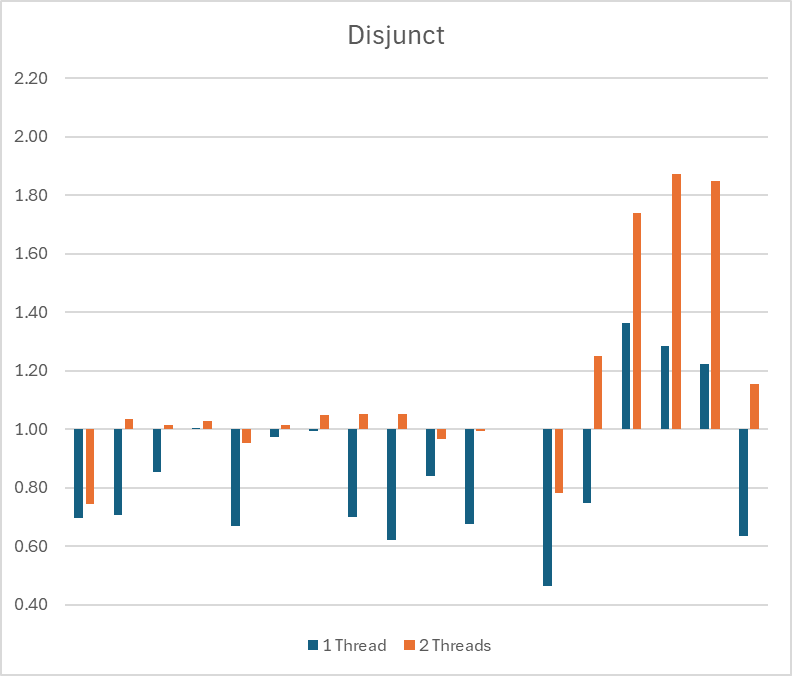
\includegraphics[width=0.5\textwidth]{../resources/Disjunct_draft.png}
    \caption[Speedup of the disjunct \ac{td}]{Speedup of the disjunct \ac{td}. The runs with a single worker thread are shown in blue, while runs with two threads are represented by orange bars. The twelve leftmost programs make up the coreutil group, while the six rightmost programs belong to the pthread group of programs}
    \label{fig:speedup_disjunct}
    % TODO: list programs
  \end{figure}

  %TODO: Dist TD shared globals!!!
  We see the disjunct \ac{td} keeping up with the baseline for most of the coreutil programs when it is run with two worker threads. Similar to the shared memory \ac{td}, it performs better on the pthread programs, where it reaches a comparatively high speedup of around 1.8 for three programs.
